\documentclass[preprint,12pt]{elsarticle}
\usepackage{amsmath}
\usepackage{booktabs}
\usepackage{graphicx}
\usepackage[colorlinks=true]{hyperref}
\graphicspath{{./figs/}}
\begin{document}
\begin{frontmatter}
\title{Supplementary Material for: Multi-Horizon Failure-Risk Models for Battery Failure Prediction: How Much Cross-Chemistry Transfer Is a State-of-Health Shortcut?}
\author{Anonymous}
\end{frontmatter}

This supplement collects the tables and figures omitted from the main text for length. All numbers are produced by the same pipeline as the main text.

\begin{table}[!t]
\caption{Calibration Quality Averaged Over Tree Models and Horizons. All Calibrators Are Fitted on Cross-Fitted Out-of-Fold Scores. Slope 1 / Intercept 0 Indicate Perfect Probabilistic Calibration.}
\label{tab:cal}
\centering
\resizebox{\textwidth}{!}{%
\begin{tabular}{llcccccc}
\toprule
\textbf{Dataset} & \textbf{Method} & \textbf{AUC (fold mean)} & \textbf{Brier} & \textbf{ECE} & \textbf{Log loss} & \textbf{Slope} & \textbf{Intercept}\\
\midrule
NASA & Isotonic & 0.854 & 0.207 & 0.151 & 0.652 & 0.48 & -0.26 \\
NASA & Platt & 0.908 & 0.196 & 0.136 & 0.575 & 0.90 & -0.14 \\
NASA & Temperature & 0.908 & 0.178 & 0.107 & 0.536 & 1.22 & -0.30 \\
CALCE & Isotonic & 0.915 & 0.067 & 0.049 & 0.279 & 0.41 & 1.17 \\
CALCE & Platt & 0.946 & 0.073 & 0.029 & 0.280 & 0.01 & 2.54 \\
CALCE & Temperature & 0.945 & 0.080 & 0.067 & 0.284 & 0.53 & 1.42 \\
\bottomrule
\end{tabular}}
\end{table}

\begin{figure}[!t]
\centering
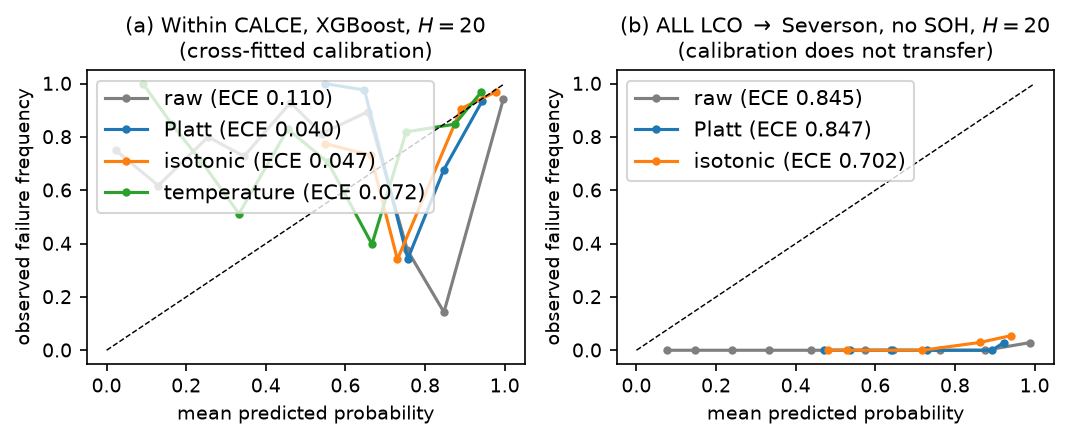
\includegraphics[width=0.9\textwidth]{fig_reliability_v2.png}
\caption{Reliability diagrams under the cross-fitted protocol. (a) Within CALCE, XGBoost at $H{=}20$: the fitted Platt sigmoid preserves ranking but washes confidence toward the base rate. (b) ALL-LCO $\to$ Severson without SOH at $H{=}20$: no fitted calibrator, whichever source scores it is applied to, repairs calibration on the shifted target.}
\label{fig:cal}
\end{figure}

\begin{figure}[!t]
\centering
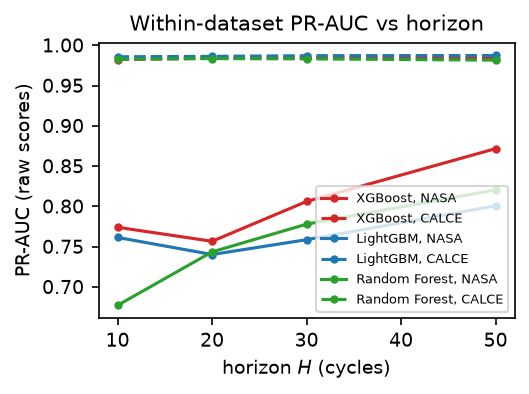
\includegraphics[width=0.65\textwidth]{fig_prauc_horizon.png}
\caption{Within-dataset PR-AUC of raw scores versus horizon. Precision--recall performance, unlike ROC-AUC, is sensitive to the horizon-dependent failure prevalence; it is also where isotonic's tied step outputs pay for their ranking-free compression.}
\label{fig:prauc}
\end{figure}

\begin{table}[!t]
\caption{GRU Transfer at H=20 on the Common Feature Set: Seed-Averaged Per-Cell AUC ($\pm$ SD Over Seeds 42, 1, 7).}
\label{tab:gru}
\centering
\small
\resizebox{\columnwidth}{!}{%
\begin{tabular}{llcc}
\toprule
\textbf{Training} & \textbf{Feature set} & \textbf{Oxford} & \textbf{Severson}\\
\midrule
NASA & common w/ SOH & 0.196$\pm$0.155 & 0.998$\pm$0.003 \\
NASA & common no SOH & 0.147$\pm$0.210 & 0.987$\pm$0.015 \\
CALCE & common w/ SOH & 0.182$\pm$0.311 & 0.964$\pm$0.033 \\
CALCE & common no SOH & 0.099$\pm$0.171 & 0.479$\pm$0.451 \\
ALL LCO & common w/ SOH & 0.088$\pm$0.084 & 0.991$\pm$0.015 \\
ALL LCO & common no SOH & 0.000$\pm$0.000 & 0.893$\pm$0.131 \\
\bottomrule
\end{tabular}}
\end{table}

\begin{table}
\centering
\caption{Minimal Transfer Baselines at H=20: Pooled AUC With Cell-Level Bootstrap 95\% CI. The Distance Rule Is the Unfitted Score $0.80-$SOH. [Oxford target].}
\label{tab:baselines-oxford}
\begin{tabular}{lccc}
\toprule
\textbf{Baseline} & \textbf{NASA} & \textbf{CALCE} & \textbf{ALL} \\
\midrule
SOH distance rule & 1.000 [1.000,1.000] & 1.000 [1.000,1.000] & 1.000 [1.000,1.000] \\
SOH only & 1.000 [1.000,1.000] & 1.000 [1.000,1.000] & 1.000 [1.000,1.000] \\
cycle only & 0.989 [0.983,1.000] & 0.756 [0.732,0.780] & 0.787 [0.760,0.814] \\
SOH + cycle & 0.990 [0.985,1.000] & 0.797 [0.770,0.825] & 0.818 [0.788,0.848] \\
sensors only & 0.500 [0.500,0.500] & 0.500 [0.500,0.500] & 0.500 [0.500,0.500] \\
full (7 feats) & 0.500 [0.500,0.500] & 0.500 [0.500,0.500] & 0.500 [0.500,0.500] \\
\bottomrule
\end{tabular}
\end{table}

\begin{table}
\centering
\caption{Minimal Transfer Baselines at H=20: Pooled AUC With Cell-Level Bootstrap 95\% CI. The Distance Rule Is the Unfitted Score $0.80-$SOH. [Severson target].}
\label{tab:baselines-severson}
\begin{tabular}{lccc}
\toprule
\textbf{Baseline} & \textbf{NASA} & \textbf{CALCE} & \textbf{ALL} \\
\midrule
SOH distance rule & 0.912 [0.836,0.998] & 0.912 [0.836,0.998] & 0.912 [0.836,0.998] \\
SOH only & 0.912 [0.836,0.998] & 0.912 [0.836,0.998] & 0.912 [0.836,0.998] \\
cycle only & 0.713 [0.591,0.798] & 0.713 [0.591,0.798] & 0.713 [0.591,0.798] \\
SOH + cycle & 0.865 [0.834,0.902] & 0.764 [0.674,0.829] & 0.758 [0.664,0.825] \\
sensors only & 0.301 [0.015,0.549] & 0.498 [0.497,0.500] & 0.303 [0.059,0.497] \\
full (7 feats) & 0.823 [0.675,0.995] & 0.712 [0.589,0.797] & 0.674 [0.525,0.782] \\
\bottomrule
\end{tabular}
\end{table}

\begin{table}
\centering
\caption{Factorial Feature Ablation at H=20 (XGBoost, Pooled AUC With Cell-Level Bootstrap 95\% CI). Feature Groups: SOH; Cycle Index; Sensors [Oxford target].}
\label{tab:abl-oxford}
\begin{tabular}{lccc}
\toprule
\textbf{Feature set} & \textbf{NASA} & \textbf{CALCE} & \textbf{ALL} \\
\midrule
Full & 0.957 [0.931,0.987] & 0.850 [0.764,0.910] & 0.917 [0.878,0.965] \\
No SOH & 0.518 [0.513,0.522] & 0.416 [0.264,0.554] & 0.429 [0.279,0.597] \\
No cycle index & 0.965 [0.942,0.989] & 0.967 [0.929,0.981] & 0.993 [0.954,1.000] \\
No SOH, no cycle & 0.658 [0.522,0.797] & 0.433 [0.282,0.594] & 0.388 [0.224,0.506] \\
SOH only & 0.965 [0.942,0.989] & 1.000 [1.000,1.000] & 1.000 [1.000,1.000] \\
Cycle only & 0.541 [0.537,0.545] & 0.541 [0.537,0.545] & 0.541 [0.537,0.545] \\
Sensors only & 0.658 [0.522,0.797] & 0.433 [0.282,0.594] & 0.388 [0.224,0.506] \\
\bottomrule
\end{tabular}
\end{table}

\begin{table}
\centering
\caption{Factorial Feature Ablation at H=20 (XGBoost, Pooled AUC With Cell-Level Bootstrap 95\% CI). Feature Groups: SOH; Cycle Index; Sensors [Severson target].}
\label{tab:abl-severson}
\begin{tabular}{lccc}
\toprule
\textbf{Feature set} & \textbf{NASA} & \textbf{CALCE} & \textbf{ALL} \\
\midrule
Full & 0.871 [0.767,0.997] & 0.850 [0.749,0.967] & 0.896 [0.812,0.995] \\
No SOH & 0.595 [0.510,0.726] & 0.682 [0.670,0.695] & 0.750 [0.692,0.835] \\
No cycle index & 0.854 [0.733,0.998] & 0.766 [0.584,0.974] & 0.774 [0.578,0.998] \\
No SOH, no cycle & 0.531 [0.433,0.680] & 0.500 [0.500,0.500] & 0.535 [0.455,0.653] \\
SOH only & 0.834 [0.695,0.991] & 0.798 [0.638,0.978] & 0.833 [0.689,0.993] \\
Cycle only & 0.709 [0.695,0.724] & 0.694 [0.681,0.708] & 0.719 [0.704,0.735] \\
Sensors only & 0.531 [0.433,0.680] & 0.500 [0.500,0.500] & 0.535 [0.455,0.653] \\
\bottomrule
\end{tabular}
\end{table}

\begin{table}[!t]
\caption{Same-Chemistry Cross-Laboratory Controls at H=20 (XGBoost, Pooled AUC [CI]). Full Feature Sets Exercise the Zero-Imputation Confound; Common Sets Restrict Both Datasets to the Shared Four-Feature Subset.}
\label{tab:samechem}
\centering
\resizebox{\textwidth}{!}{%
\begin{tabular}{lccc}
\toprule
\textbf{Pair} & \textbf{with SOH (full)} & \textbf{no SOH (full)} & \textbf{no SOH (common)}\\
\midrule
NASA$\to$CALCE (LCO$\to$LCO) & 0.870 [0.799,0.966] & 0.849 [0.753,0.985] & 0.781 [0.708,0.964] \\
CALCE$\to$NASA (LCO$\to$LCO) & 0.543 [0.356,0.677] & 0.566 [0.427,0.678] & 0.601 [0.496,0.703] \\
Severson$\to$Oxford (LFP$\to$LFP) & 0.997 [0.991,1.000] & 0.471 [0.466,0.477] & 0.428 [0.422,0.435] \\
Oxford$\to$Severson (LFP$\to$LFP) & 0.688 [0.605,0.788] & 0.500 [0.500,0.500] & 0.500 [0.500,0.500] \\
\bottomrule
\end{tabular}}
\end{table}

\begin{table}[!t]
\caption{Discrete-Time Hazard Model at H=20: Transfer Performance (Pooled AUC [CI]). The Fixed-Horizon XGBoost Comparator With SOH Is in main-text Table 3.}
\label{tab:hazard}
\centering
\resizebox{\textwidth}{!}{%
\begin{tabular}{llcc}
\toprule
\textbf{Training} & \textbf{Model} & \textbf{Oxford} & \textbf{Severson}\\
\midrule
NASA & Hazard XGBoost & 0.971 [0.953,0.991] & 0.884 [0.786,0.998] \\
NASA & Hazard Logistic & 0.500 [0.500,0.500] & 0.607 [0.402,0.890] \\
CALCE & Hazard XGBoost & 0.466 [0.301,0.578] & 0.737 [0.711,0.774] \\
CALCE & Hazard Logistic & 0.500 [0.500,0.500] & 0.500 [0.500,0.500] \\
ALL LCO & Hazard XGBoost & 0.314 [0.135,0.457] & 0.866 [0.770,0.978] \\
ALL LCO & Hazard Logistic & 0.500 [0.500,0.500] & 0.916 [0.873,0.969] \\
\bottomrule
\end{tabular}}
\end{table}

\begin{table}[!t]
\caption{Monotonicity Violations: Share of Scored Rows With $p_{10}\le p_{20}\le p_{30}\le p_{50}$ Failing, on Raw Scores (Platt in Parentheses). The Survival Product Is Monotone by Construction (Rate 0).}
\label{tab:mono}
\centering
\resizebox{\columnwidth}{!}{%
\begin{tabular}{lllcc}
\toprule
\textbf{Setting} & \textbf{Target} & \textbf{Model} & \textbf{Raw} & \textbf{Platt}\\
\midrule
within & calce & XGBoost & 0.452 & 0.056 \\
within & nasa & XGBoost & 0.323 & 0.260 \\
transfer (calce src) & oxford & LightGBM & 0.641 & 0.004 \\
transfer (calce src) & oxford & Random Forest & 0.501 & 0.540 \\
transfer (calce src) & oxford & XGBoost & 0.565 & 0.003 \\
transfer (nasa+calce src) & oxford & LightGBM & 0.210 & 0.648 \\
transfer (nasa+calce src) & oxford & Random Forest & 0.335 & 0.305 \\
transfer (nasa+calce src) & oxford & XGBoost & 0.609 & 0.341 \\
transfer (nasa src) & oxford & LightGBM & 0.521 & 0.468 \\
transfer (nasa src) & oxford & Random Forest & 0.559 & 0.376 \\
transfer (nasa src) & oxford & XGBoost & 0.248 & 0.124 \\
transfer (calce src) & severson & LightGBM & 0.405 & 0.013 \\
transfer (calce src) & severson & XGBoost & 0.420 & 0.072 \\
transfer (nasa src) & severson & LightGBM & 0.582 & 0.537 \\
transfer (nasa src) & severson & Random Forest & 0.778 & 0.557 \\
transfer (nasa src) & severson & XGBoost & 0.958 & 0.923 \\
--- & --- & Survival product & 0.000 & 0.000 \\
\bottomrule
\end{tabular}}
\end{table}

\begin{table}[!t]
\caption{Arm A Recalibration on Severson Without SOH ($H{=}20$): Values Average the Three LCO Sources and Available Tree Models; ECE Uses 10 Equal-Width Probability Bins. From the Released Recalibration Study Artifacts.}
\label{tab:rec-r1}
\centering
\resizebox{\textwidth}{!}{%
\begin{tabular}{rccccccc}
\toprule
$k$ & Zero ECE & Iso. ECE & Platt ECE & Temp. ECE & Iso. AUC & Platt AUC & Temp. AUC\\
\midrule
5 & 0.817 & 0.044 & 0.045 & 0.563 & 0.616 & 0.599 & 0.669 \\
10 & 0.817 & 0.010 & 0.010 & 0.561 & 0.634 & 0.646 & 0.651 \\
20 & 0.817 & 0.013 & 0.013 & 0.560 & 0.634 & 0.655 & 0.648 \\
40 & 0.817 & 0.015 & 0.015 & 0.561 & 0.637 & 0.657 & 0.653 \\
\bottomrule
\end{tabular}}
\end{table}

\begin{table}[!t]
\caption{Arm B Recovery at $k=5$ on Severson Without SOH, $H=20$. Recovery Ratio Uses the Within-LCO Ceiling; Retention Is the LCO-Holdout AUC Before and After the Update. \textsuperscript{*}Ratio above 1.0 is a ceiling-mismatch artifact, not super-ceiling recovery (see text).}
\label{tab:rec-r2}
\centering
\resizebox{\textwidth}{!}{%
\begin{tabular}{llccccc}
\toprule
\textbf{Training} & \textbf{Model} & \textbf{Zero AUC} & \textbf{Arm B AUC} & \textbf{Recovery} & \textbf{DeLong p} & \textbf{LCO retention}\\
\midrule
NASA & XGBoost & 0.620 & 0.854 & +1.04\textsuperscript{*} & $<10^{-3}$ & 1.000 $\rightarrow$ 1.000 \\
NASA & LightGBM & 0.493 & 0.838 & +0.88 & $<10^{-3}$ & 1.000 $\rightarrow$ 0.997 \\
NASA & Random Forest & 0.724 & 0.751 & +0.19 & $<10^{-3}$ & 0.959 $\rightarrow$ 0.314 \\
CALCE & XGBoost & 0.686 & 0.796 & +0.53 & $<10^{-3}$ & 0.997 $\rightarrow$ 0.996 \\
ALL LCO & XGBoost & 0.760 & 0.828 & +0.47 & $<10^{-3}$ & 0.690 $\rightarrow$ 0.567 \\
\bottomrule
\end{tabular}}
\end{table}

\begin{table}[!t]
\caption{SOH Ablation Evidence (ALL-LCO Source): Pooled AUC With and Without SOH, Paired Cell-Level Bootstrap 95\% CI on the Difference (Primary), and Cycle-Level DeLong $p$-Value (Secondary; Inflated by Within-Cell Correlation).}
\label{tab:sohtests}
\centering
\resizebox{\textwidth}{!}{%
\begin{tabular}{llccccc}
\toprule
\textbf{Target} & \textbf{Model} & \textbf{H} & \textbf{AUC w/ SOH} & \textbf{AUC w/o} & \textbf{Delta AUC [boot 95\% CI]} & \textbf{DeLong p}\\
\midrule
Oxford & XGBoost & 10 & 0.980 & 0.433 & +0.547 (CI undefined: 5 cells) & $<10^{-16}$ (underflow) \\
Oxford & XGBoost & 20 & 0.917 & 0.429 & +0.488 (CI undefined: 5 cells) & $<10^{-16}$ (underflow) \\
Oxford & XGBoost & 30 & 0.991 & 0.377 & +0.614 (CI undefined: 5 cells) & $<10^{-16}$ (underflow) \\
Oxford & XGBoost & 50 & 0.932 & 0.580 & +0.351 (CI undefined: 5 cells) & $<10^{-16}$ (underflow) \\
Oxford & LightGBM & 10 & 0.996 & 0.547 & +0.449 (CI undefined: 5 cells) & $<10^{-16}$ (underflow) \\
Oxford & LightGBM & 20 & 0.971 & 0.332 & +0.639 (CI undefined: 5 cells) & $<10^{-16}$ (underflow) \\
Oxford & LightGBM & 30 & 0.743 & 0.484 & +0.259 (CI undefined: 5 cells) & $9.7e-13$ \\
Oxford & LightGBM & 50 & 0.832 & 0.448 & +0.384 (CI undefined: 5 cells) & $<10^{-16}$ (underflow) \\
Oxford & Random Forest & 10 & 0.978 & 0.626 & +0.352 (CI undefined: 5 cells) & $<10^{-16}$ (underflow) \\
Oxford & Random Forest & 20 & 0.989 & 0.581 & +0.409 (CI undefined: 5 cells) & $<10^{-16}$ (underflow) \\
Oxford & Random Forest & 30 & 0.971 & 0.462 & +0.508 (CI undefined: 5 cells) & $<10^{-16}$ (underflow) \\
Oxford & Random Forest & 50 & 0.933 & 0.460 & +0.473 (CI undefined: 5 cells) & $<10^{-16}$ (underflow) \\
Severson & XGBoost & 10 & 0.878 & 0.741 & +0.137 [0.079, 0.249] & $<10^{-16}$ (underflow) \\
Severson & XGBoost & 20 & 0.896 & 0.750 & +0.146 [0.097, 0.233] & $<10^{-16}$ (underflow) \\
Severson & XGBoost & 30 & 0.906 & 0.745 & +0.162 [0.115, 0.237] & $<10^{-16}$ (underflow) \\
Severson & XGBoost & 50 & 0.917 & 0.736 & +0.180 [0.134, 0.250] & $<10^{-16}$ (underflow) \\
Severson & LightGBM & 10 & 0.870 & 0.736 & +0.134 [0.105, 0.200] & $<10^{-16}$ (underflow) \\
Severson & LightGBM & 20 & 0.882 & 0.718 & +0.164 [0.127, 0.227] & $<10^{-16}$ (underflow) \\
Severson & LightGBM & 30 & 0.872 & 0.771 & +0.102 [0.030, 0.230] & $<10^{-16}$ (underflow) \\
Severson & LightGBM & 50 & 0.899 & 0.744 & +0.155 [0.112, 0.214] & $<10^{-16}$ (underflow) \\
Severson & Random Forest & 10 & 0.903 & 0.740 & +0.163 [0.133, 0.225] & $<10^{-16}$ (underflow) \\
Severson & Random Forest & 20 & 0.889 & 0.746 & +0.143 [0.106, 0.226] & $<10^{-16}$ (underflow) \\
Severson & Random Forest & 30 & 0.919 & 0.748 & +0.171 [0.138, 0.232] & $<10^{-16}$ (underflow) \\
Severson & Random Forest & 50 & 0.921 & 0.746 & +0.175 [0.114, 0.264] & $<10^{-16}$ (underflow) \\
\bottomrule
\end{tabular}}
\end{table}

\begin{figure}[!t]
\centering
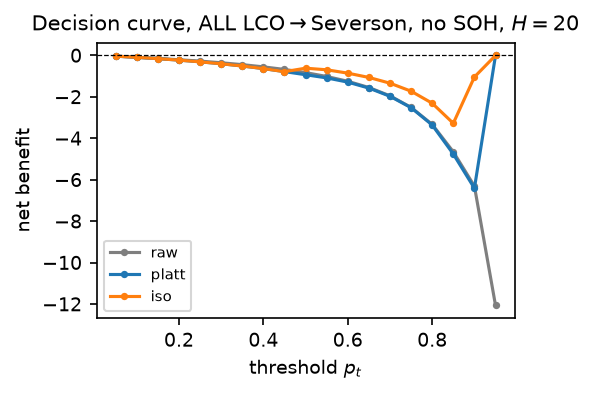
\includegraphics[width=0.75\textwidth]{fig_netbenefit.png}
\caption{Decision-curve analysis (net benefit vs.\ threshold) for ALL-LCO $\to$ Severson without SOH at $H{=}20$: no score type produces a usable operating point once SOH is removed.}
\label{fig:netbenefit}
\end{figure}

\begin{figure}[!t]
\centering
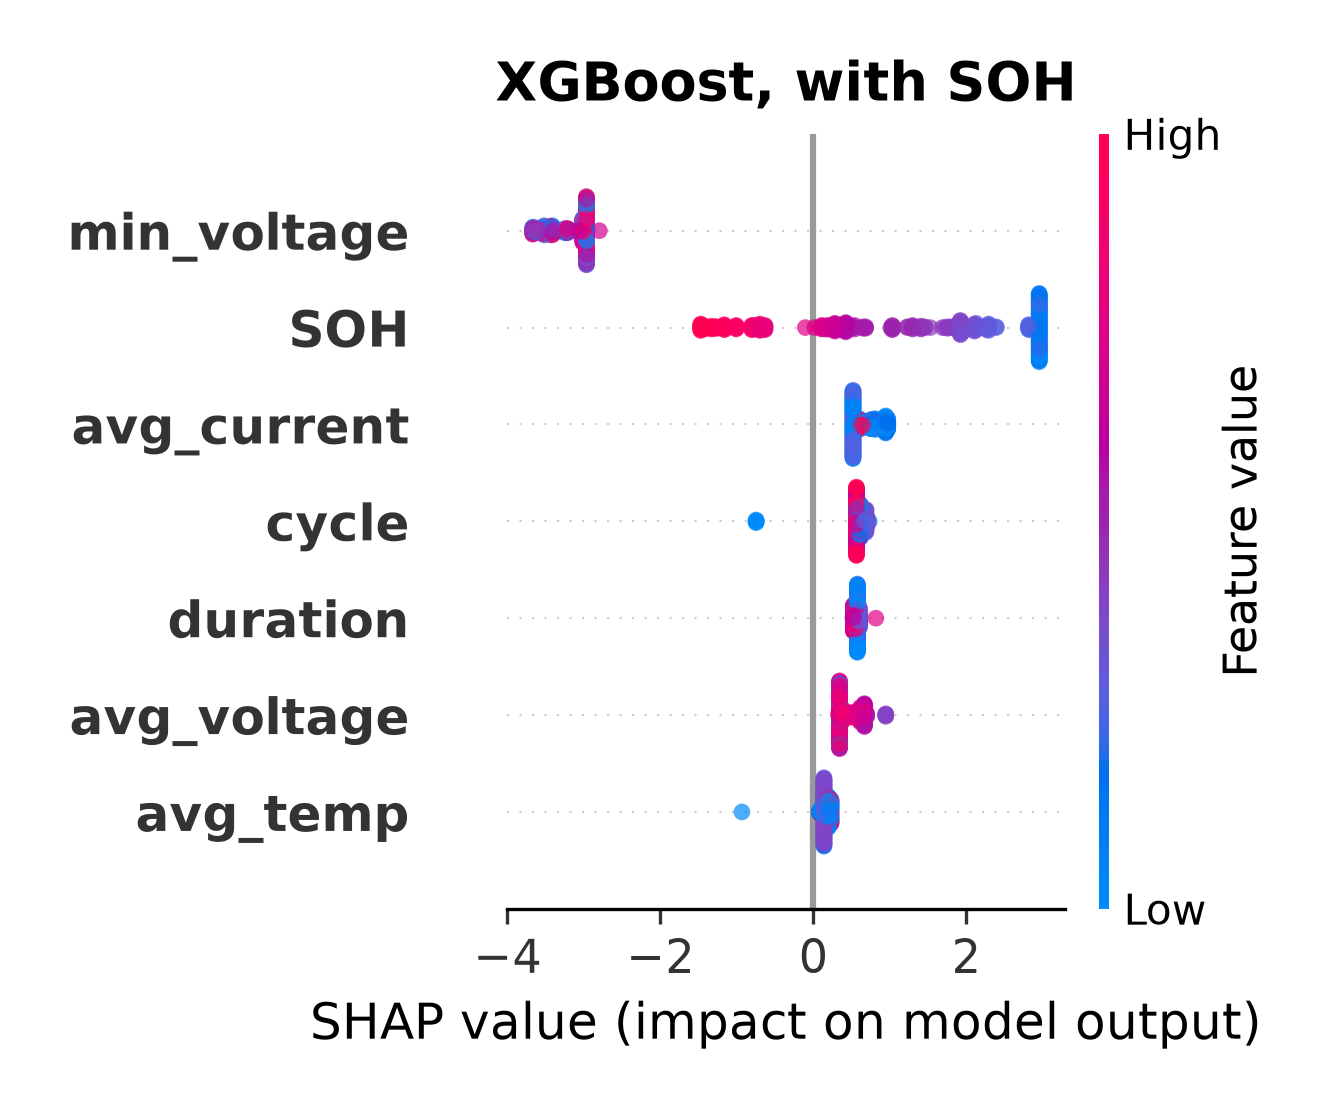
\includegraphics[width=0.85\textwidth]{Fig06a_XGBoost_SHAP.png}
\caption{SHAP feature importance for XGBoost in NASA-to-Oxford transfer at H=20, with SOH. SOH dominates by a wide margin.}
\label{fig:shap_xgb}
\end{figure}

\begin{figure}[!t]
\centering
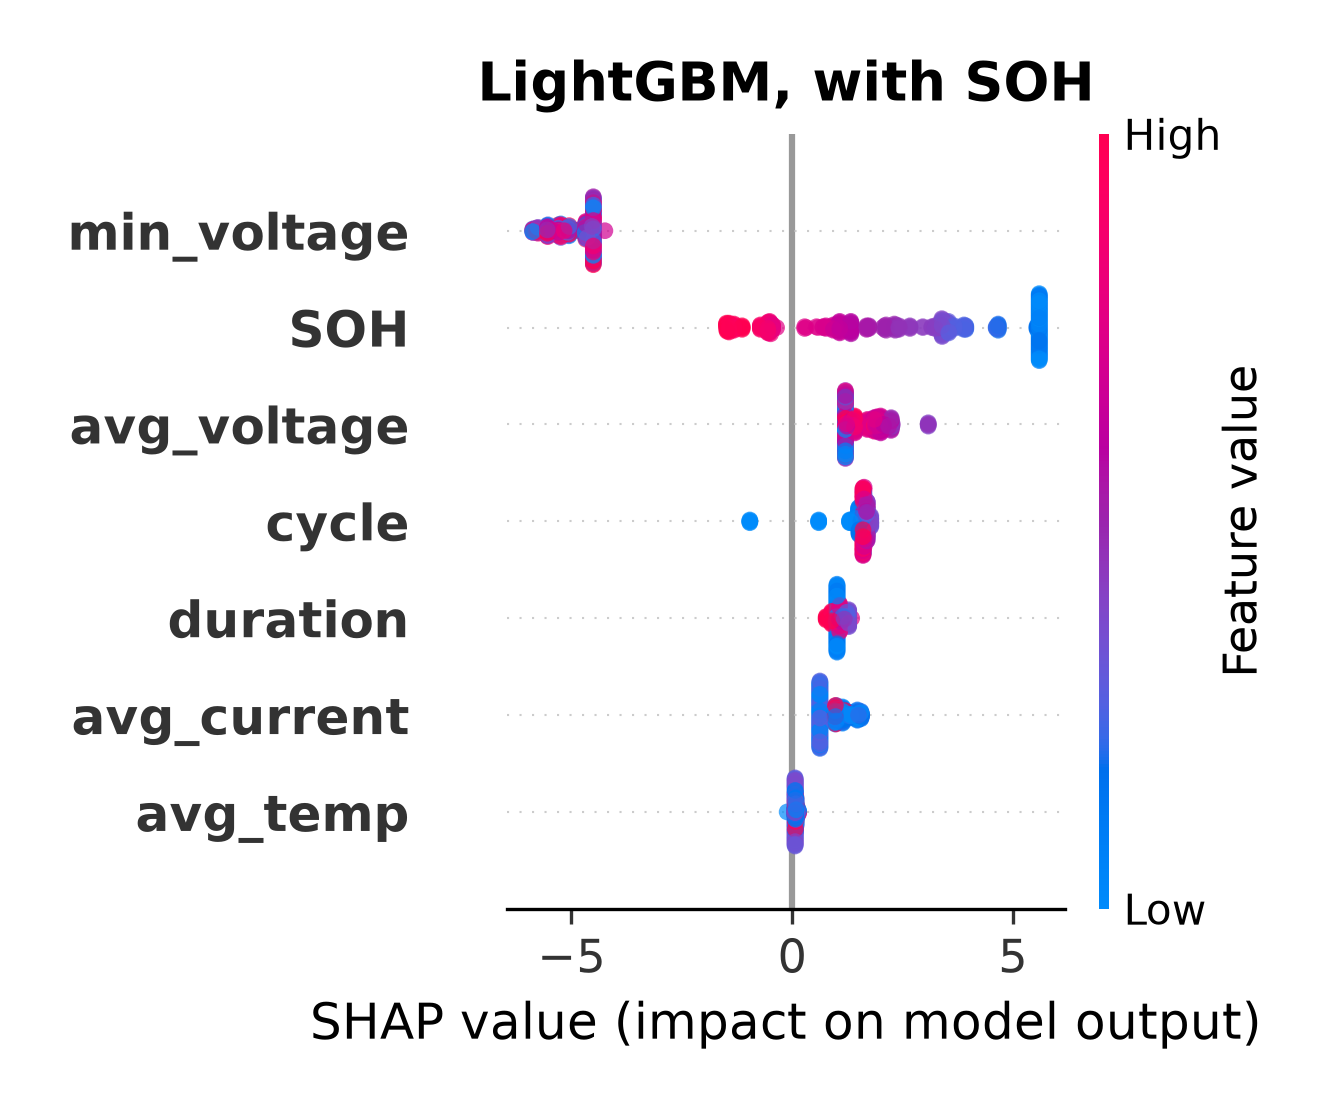
\includegraphics[width=0.85\textwidth]{Fig06b_LightGBM_SHAP.png}
\caption{SHAP feature importance for LightGBM in NASA-to-Oxford transfer at H=20, with SOH. SOH dominates by a wide margin.}
\label{fig:shap_lgbm}
\end{figure}

\begin{figure}[!t]
\centering
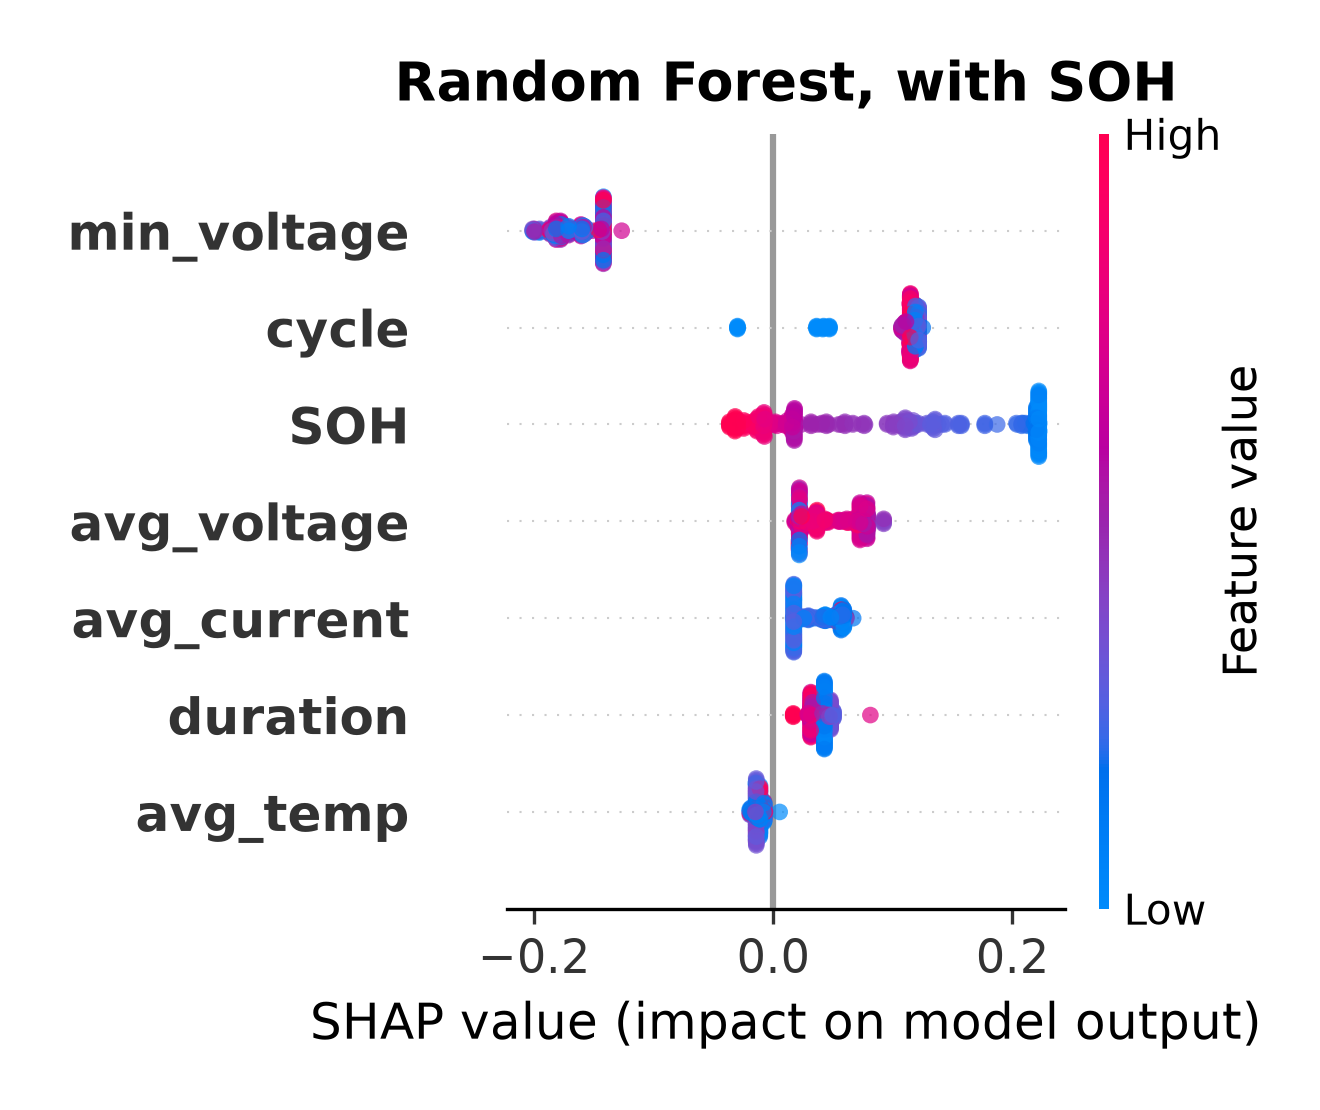
\includegraphics[width=0.85\textwidth]{Fig06c_RandomForest_SHAP.png}
\caption{SHAP feature importance for Random Forest in NASA-to-Oxford transfer at H=20, with SOH. SOH dominates by a wide margin.}
\label{fig:shap_rf}
\end{figure}

\begin{figure}[!t]
\centering
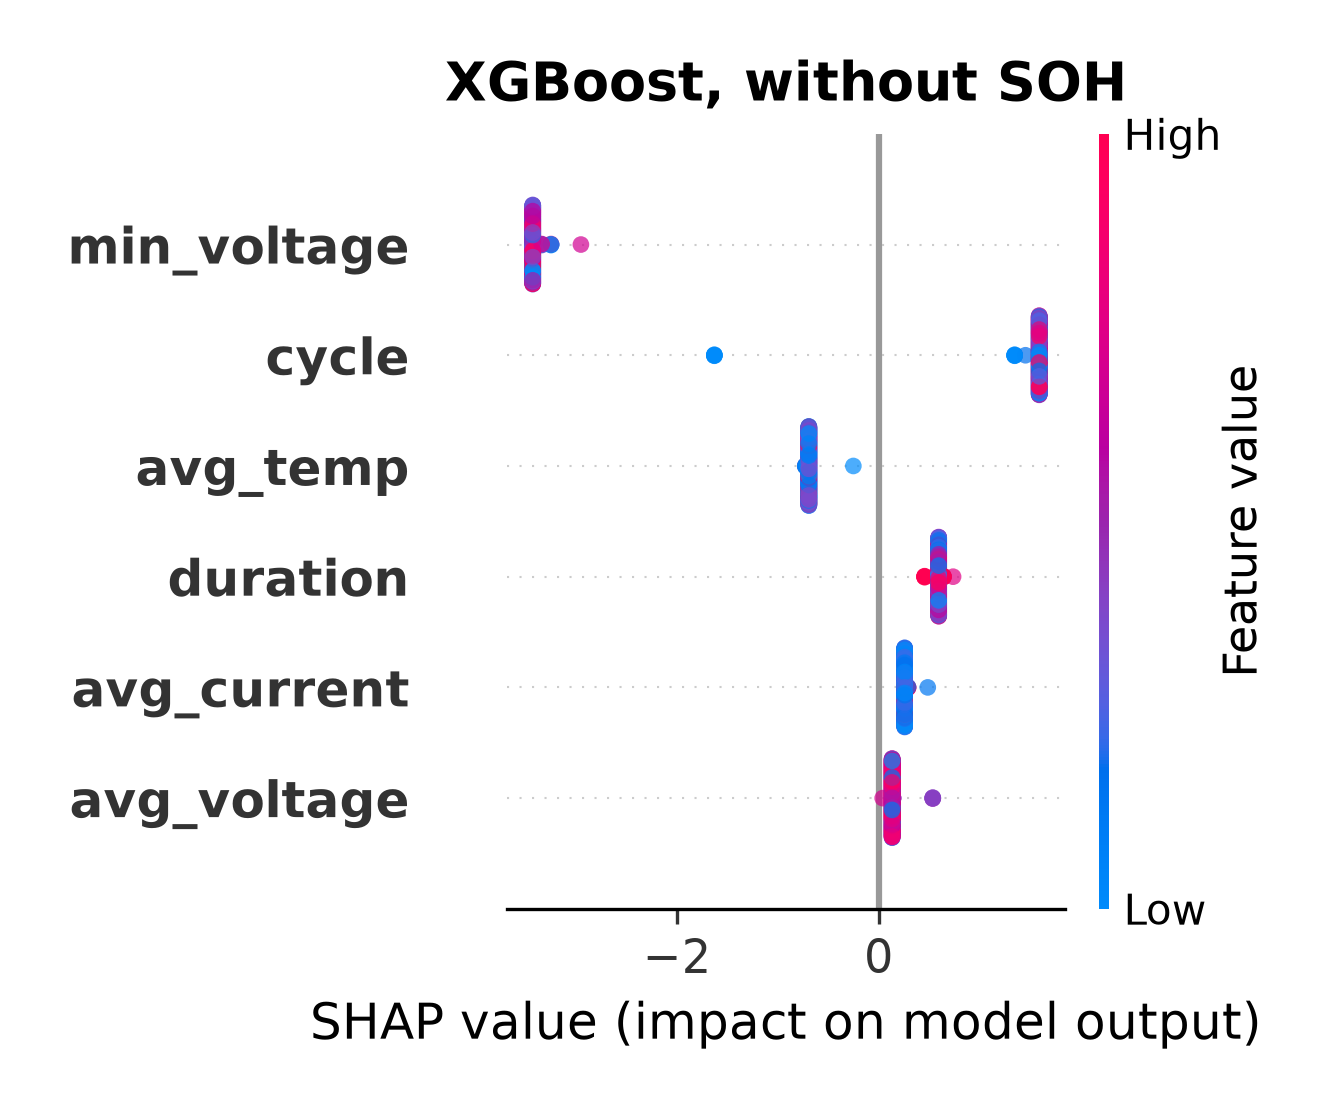
\includegraphics[width=0.85\textwidth]{Fig06d_XGBoost_SHAP_noSOH.png}
\caption{SHAP feature importance for XGBoost in NASA-to-Oxford transfer at H=20, without SOH. All features collapse to near-zero spread, so no transferable signal remains.}
\label{fig:shap_noxgb}
\end{figure}

\begin{figure}[!t]
\centering
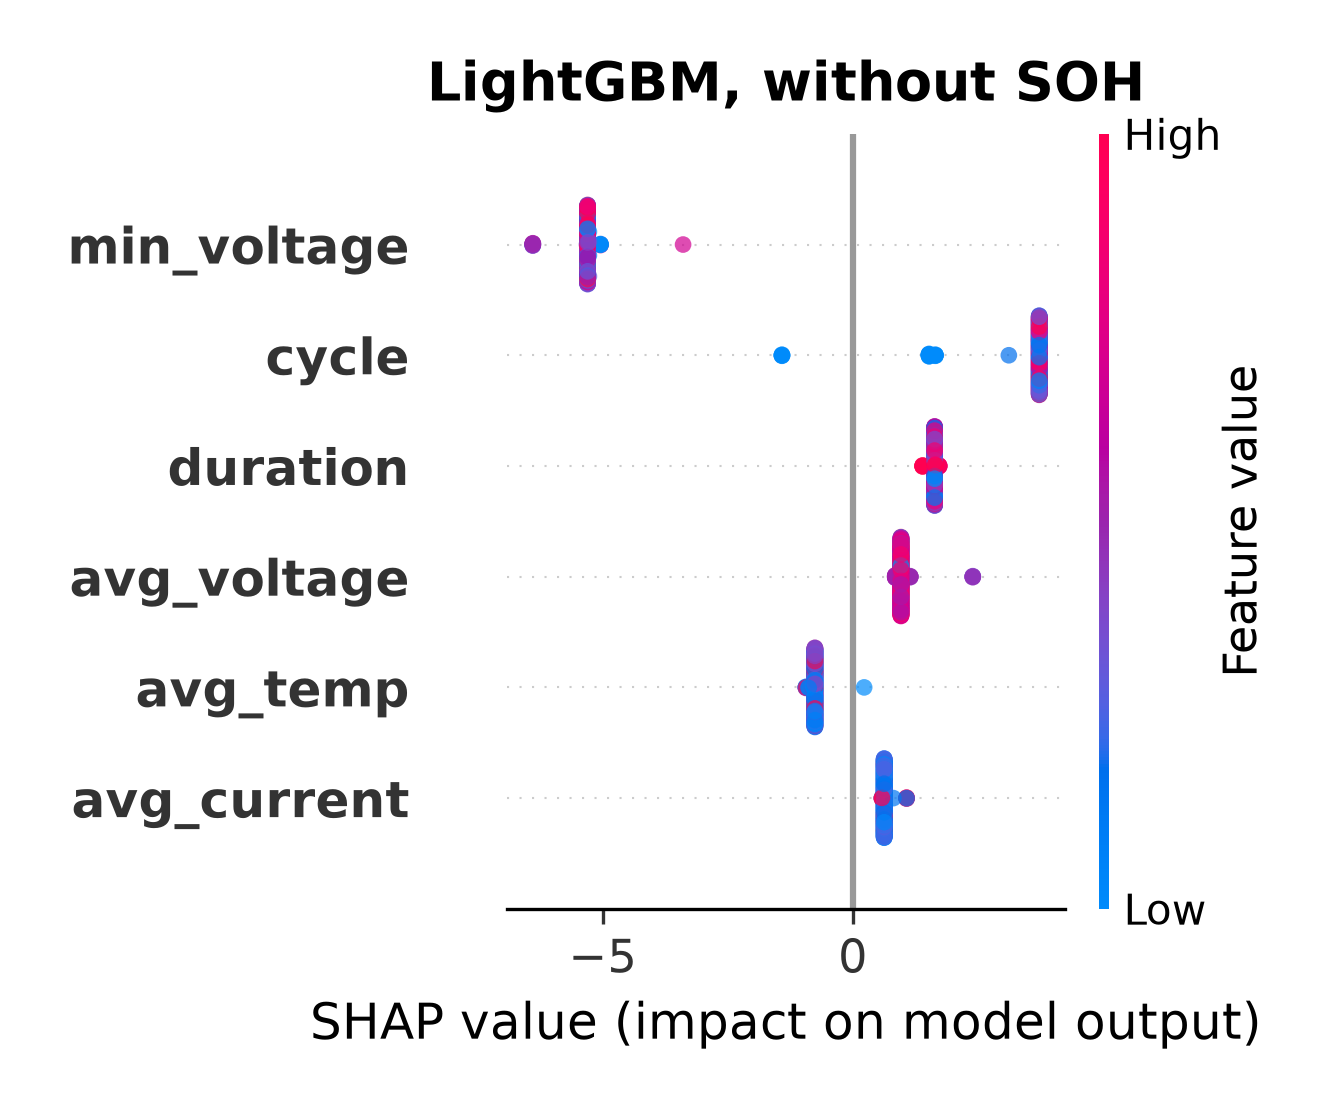
\includegraphics[width=0.85\textwidth]{Fig06e_LightGBM_SHAP_noSOH.png}
\caption{SHAP feature importance for LightGBM in NASA-to-Oxford transfer at H=20, without SOH. All features collapse to near-zero spread.}
\label{fig:shap_nolgbm}
\end{figure}

\begin{figure}[!t]
\centering
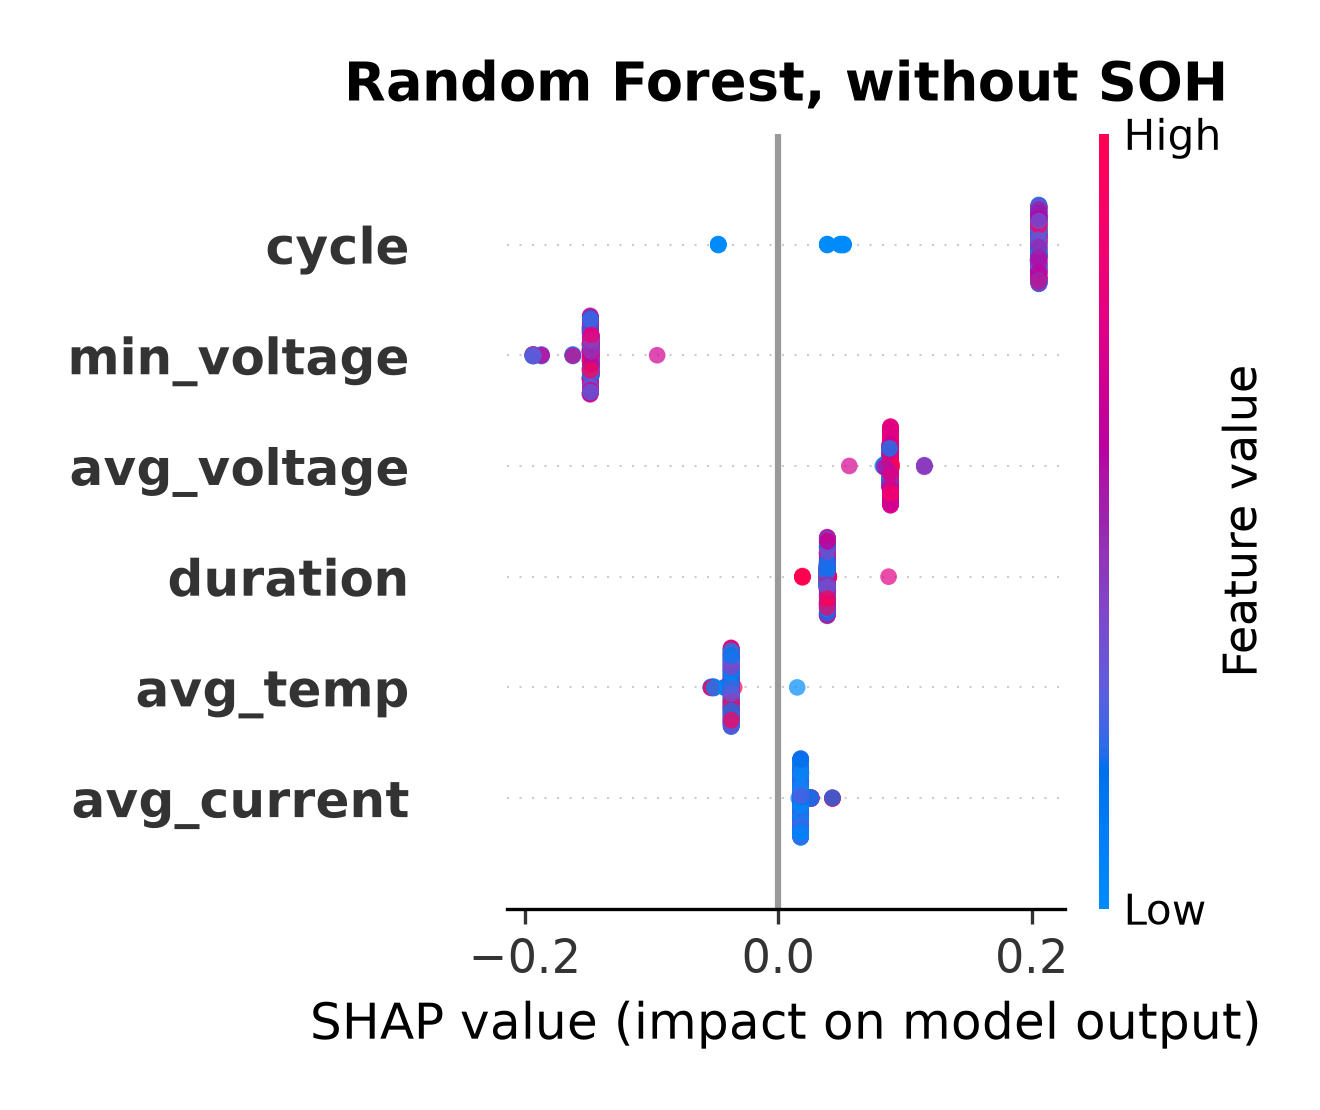
\includegraphics[width=0.85\textwidth]{Fig06f_RandomForest_SHAP_noSOH.png}
\caption{SHAP feature importance for Random Forest in NASA-to-Oxford transfer at H=20, without SOH. All features collapse to near-zero spread.}
\label{fig:shap_norf}
\end{figure}

\begin{table}[!t]
\caption{Embedded Deployment: Model Size, Accuracy, On-Device Validation Error, and Measured Inference Time. Errors Are Maximum $|$C engine $-$ \texttt{predict\_proba()}$|$ Over All 1 028 Rows. Timings Measured On-Device at 240 MHz With the Binary in Flash (PROGMEM), PSRAM, or a Single Model in Internal SRAM.}
\label{tab:deploy}
\centering
\resizebox{\textwidth}{!}{%
\begin{tabular}{lccccc}
\toprule
\textbf{Model} & \textbf{Nodes} & \textbf{Max Err} & \textbf{Flash} & \textbf{PSRAM} & \textbf{SRAM (1 model)}\\
\midrule
XGBoost & 3 272 & $2.4\times10^{-7}$ & 0.76 ms & 0.50 ms & 0.32 ms\\
LightGBM & 7 000 & $1.1\times10^{-6}$ & 1.55 ms & 0.93 ms & 0.43 ms\\
Random Forest & 16 064 & $3.0\times10^{-8}$ & 2.36 ms & 1.29 ms & 0.50 ms\\
All three & 26 336 & --- & 4.7 ms & 2.7 ms & ---\\
\bottomrule
\end{tabular}}
\end{table}

\begin{figure}[!t]
\centering
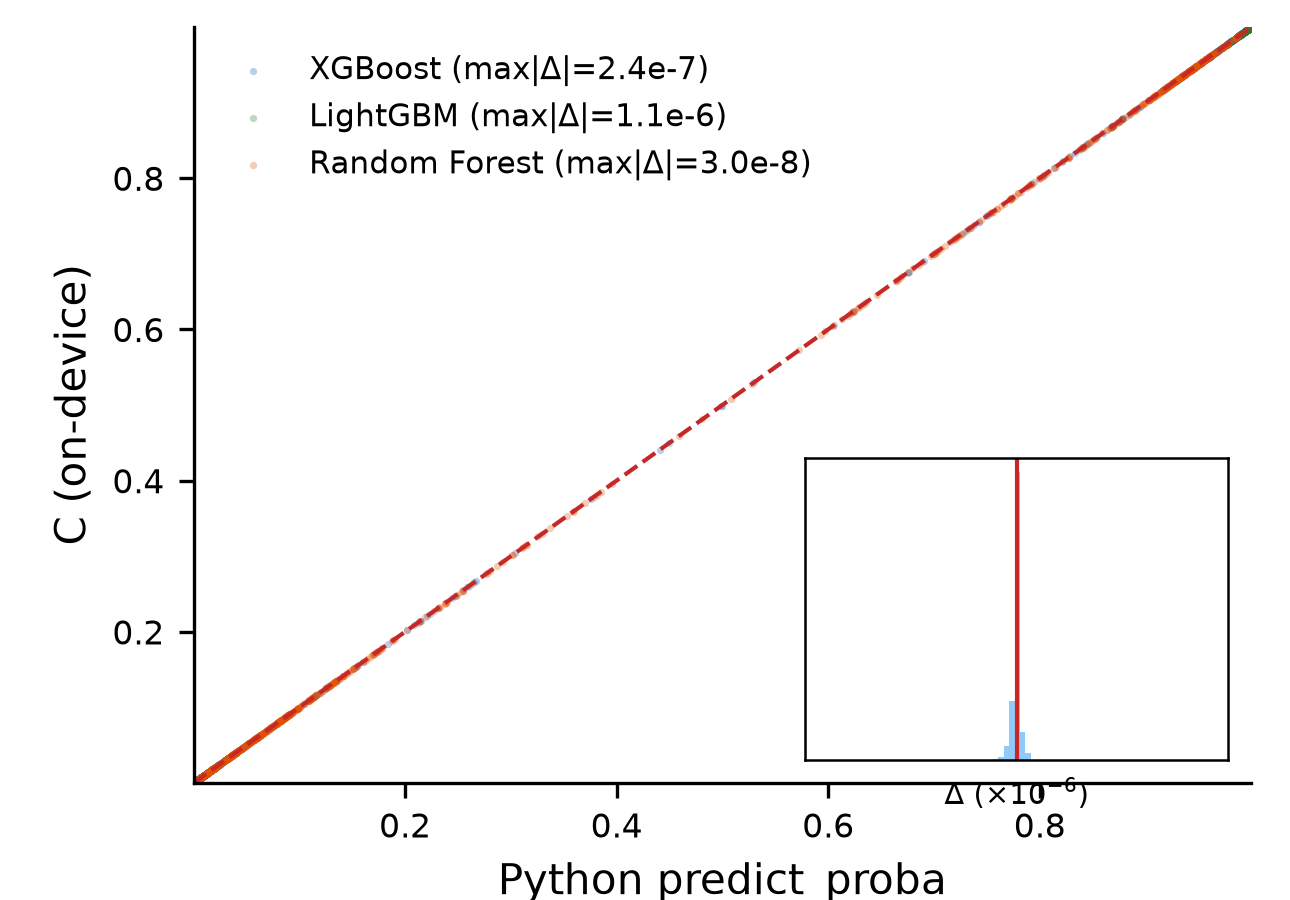
\includegraphics[width=0.9\textwidth]{fig_py_c_agreement.png}
\caption{On-device C engine predictions versus Python \texttt{predict\_proba()} over all 1 028 rows and three models (agreement scatter on the identity line, inset residual histogram of C minus Python in units of $10^{-6}$). Maximum absolute errors are $2.4\times10^{-7}$ (XGBoost), $1.1\times10^{-6}$ (LightGBM), and $3.0\times10^{-8}$ (Random Forest).}
\label{fig:pyc}
\end{figure}

\begin{table}[!t]
\caption{Transfer to New Chemistries at H=20 (NASA+CALCE Source). Pooled AUC With Cell-Level Bootstrap 95\% CI; $\Delta$ Is the Paired Per-Cell Bootstrap Difference (With $-$ Without SOH). New Groups Are Transfer Targets Only.}
\label{tab:crosschemnew}
\centering
\resizebox{\textwidth}{!}{%
\begin{tabular}{llccc}
\toprule
\textbf{Target} & \textbf{Model} & \textbf{With SOH} & \textbf{Without SOH} & \textbf{Delta (paired)}\\
\midrule
HNEI NMC & XGBoost & 0.993 [0.983,0.999] & 0.989 [0.977,0.997] & +0.004  \\
HNEI NMC & LightGBM & 0.999 [0.998,0.999] & 0.988 [0.974,0.996] & +0.011  \\
HNEI NMC & Random Forest & 0.999 [0.999,1.000] & 0.996 [0.994,0.999] & +0.003  \\
SNL NCA & XGBoost & 0.972 [0.956,0.988] & 0.878 [0.824,0.930] & +0.094  \\
SNL NCA & LightGBM & 0.985 [0.974,0.993] & 0.850 [0.791,0.911] & +0.135  \\
SNL NCA & Random Forest & 0.983 [0.974,0.992] & 0.911 [0.875,0.951] & +0.072  \\
SNL NMC & XGBoost & 0.772 [0.677,0.979] & 0.709 [0.612,0.953] & +0.063  \\
SNL NMC & LightGBM & 0.847 [0.743,0.982] & 0.693 [0.570,0.959] & +0.153  \\
SNL NMC & Random Forest & 0.858 [0.748,0.975] & 0.742 [0.689,0.874] & +0.115  \\
SNL LFP & XGBoost & 0.998 [0.997,1.000] & 0.496 [0.458,0.531] & +0.502  \\
SNL LFP & LightGBM & 0.999 [0.997,1.000] & 0.359 [0.279,0.443] & +0.640  \\
SNL LFP & Random Forest & 0.999 [0.998,1.000] & 0.666 [0.569,0.769] & +0.332  \\
\bottomrule
\end{tabular}}
\end{table}

\begin{figure}[!t]
\centering
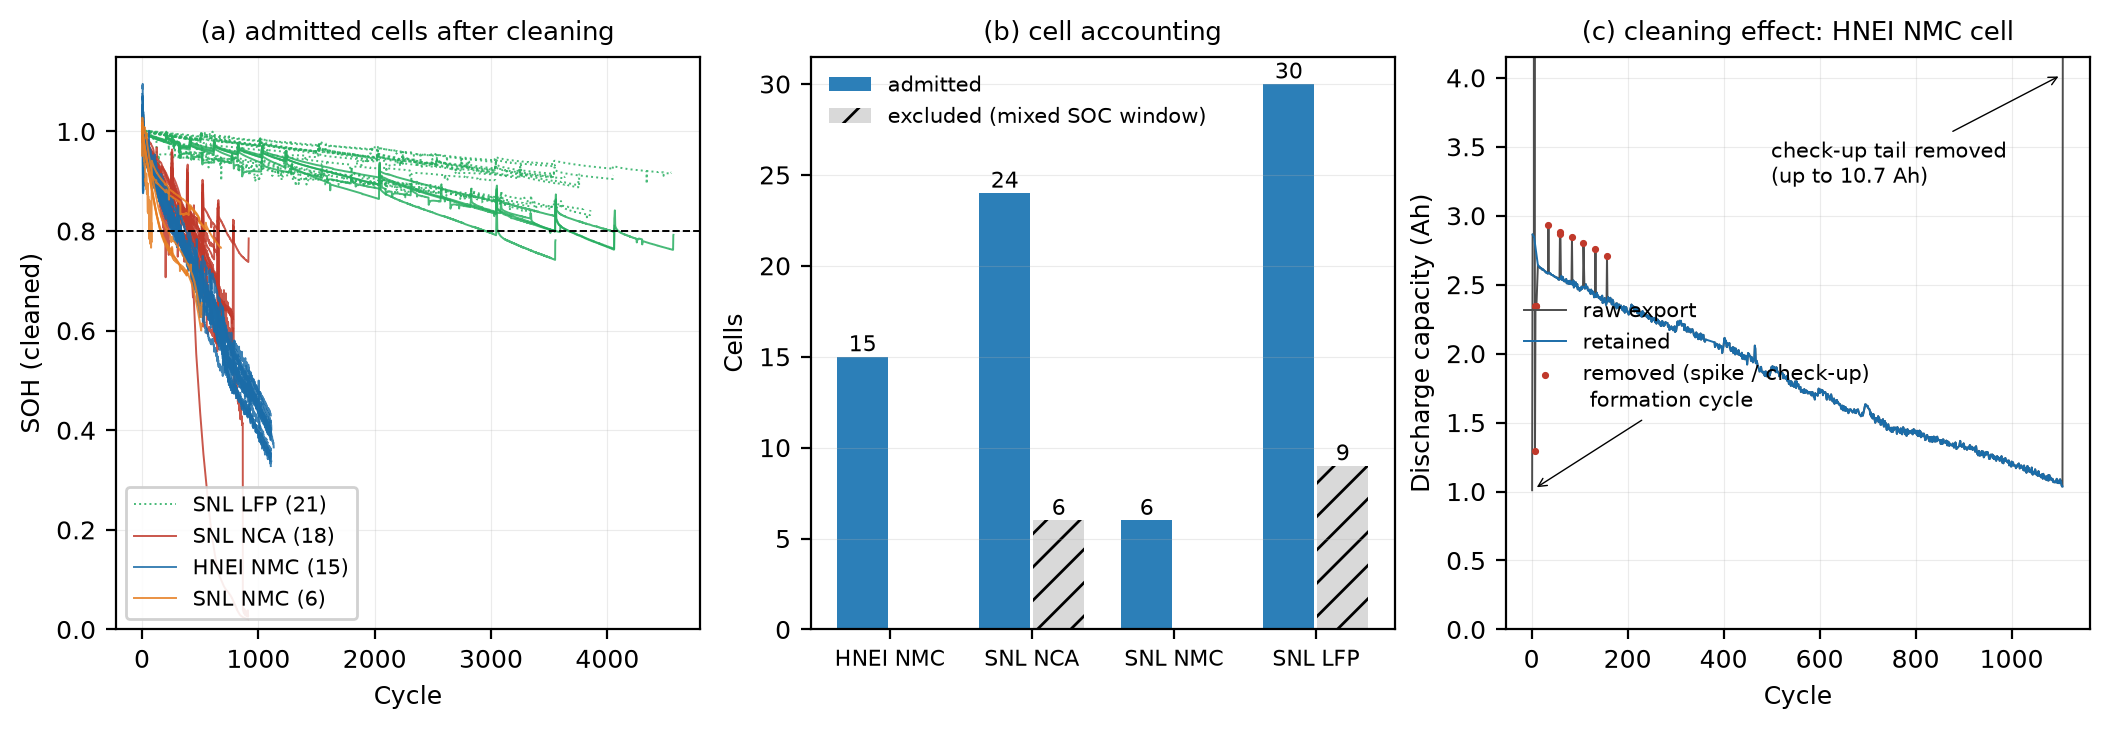
\includegraphics[width=0.95\textwidth]{fig_ba_quality.png}
\caption{Data audit of the Battery Archive groups after the pre-registered cleaning rule (formation-cycle drop, Hampel despiking, level-shift truncation, voltage validity, minimum 20 usable cycles): (a) admitted-cell capacity traces with the 80\% end-of-life criterion; (b) retained versus excluded cycles per group; (c) recorded exclusion reasons. Of 75 downloaded cells, 60 are admitted and 15 are excluded for exactly one recorded reason.}
\label{fig:baquality}
\end{figure}

\begin{table}[!t]
\caption{Leave-Condition-Out Versus Mixed-Cell Folds at H=20 (XGBoost). Conditions Are Temperature Band, C-Rate, or Both; Metadata Never Enters the Features. Ref.\ Is the Ordinary Mixed-Cell AUC for the Same Feature Set (--- Where Unstable or Not Run).}
\label{tab:condshift}
\centering
\resizebox{\columnwidth}{!}{%
\begin{tabular}{llcccc}
\toprule
\textbf{Group} & \textbf{Held-out axis} & \textbf{With SOH} & \textbf{Ref.} & \textbf{No SOH} & \textbf{Ref.}\\
\midrule
SNL NCA & temp $\times$ rate & 0.989  & 0.985 & 0.894  & 0.928 \\
SNL NCA & temperature & 0.989  & 0.985 & 0.888  & 0.928 \\
SNL NCA & C-rate & 0.961  & 0.985 & 0.820  & 0.928 \\
SNL NMC & temp $\times$ rate & 0.847  & --- & 0.666  & --- \\
SNL NMC & temperature & 0.787  & --- & 0.569  & --- \\
SNL NMC & C-rate & 0.847  & --- & 0.666  & --- \\
SNL LFP & temp $\times$ rate & 0.991  & 0.994 & --- & --- \\
SNL LFP & temperature & 0.995  & 0.994 & --- & --- \\
SNL LFP & C-rate & 0.994  & 0.994 & --- & --- \\
\bottomrule
\end{tabular}}
\end{table}
\begin{thebibliography}{99}
\bibitem{meng2019review} H. Meng and Y. Li, ``A review on prognostics and health management (PHM) methods of lithium-ion batteries,'' \emph{Renew. Sustain. Energy Rev.}, vol. 116, Art. no. 109405, 2019.
\bibitem{roman2021machine} D. Roman, S. Saxena, V. Robu, et al., ``Machine learning pipeline for battery state-of-health estimation,'' \emph{Nat. Mach. Intell.}, vol. 3, no. 4, pp. 447--456, 2021.
\bibitem{sulzer2021challenge} V. Sulzer, P. Mohtat, A. Aitio, et al., ``The challenge and opportunity of battery lifetime prediction from field data,'' \emph{Joule}, vol. 5, no. 8, pp. 1934--1955, 2021.
\bibitem{breiman2001random} L. Breiman, ``Random forests,'' \emph{Mach. Learn.}, vol. 45, no. 1, pp. 5--32, 2001.
\bibitem{chen2016xgboost} T. Chen and C. Guestrin, ``XGBoost: A scalable tree boosting system,'' in \emph{Proc. ACM SIGKDD}, 2016, pp. 785--794.
\bibitem{ke2017lightgbm} G. Ke, Q. Meng, T. Finley, et al., ``LightGBM: A highly efficient gradient boosting decision tree,'' in \emph{Proc. NeurIPS}, vol. 30, 2017, pp. 3146--3154.
\bibitem{shikdar2026learning} T. A. Shikdar and H. Laaksonen, ``Learning when not to use a battery: Multihorizon failure intelligence,'' \emph{Int. Trans. Electr. Energy Syst.}, vol. 36, Art. no. 6000810, 2026.
\bibitem{sahoo2022transfer} S. Sahoo, K. S. Hariharan, S. Agarwal, et al., ``Transfer learning based generalized framework for state of health estimation of Li-ion cells,'' \emph{Sci. Rep.}, vol. 12, Art. no. 13173, 2022.
\bibitem{lu2023deep} J. Lu, R. Xiong, J. Tian, C. Wang, and F. Sun, ``Deep learning to estimate lithium-ion battery state of health without additional degradation experiments,'' \emph{Nat. Commun.}, vol. 14, Art. no. 2760, 2023.
\bibitem{platt1999probabilistic} J. C. Platt, ``Probabilistic outputs for support vector machines and comparisons to regularized likelihood methods,'' in \emph{Adv. Large Margin Classifiers}, MIT Press, 1999, pp. 61--74.
\bibitem{zadrozny2002transforming} B. Zadrozny and C. Elkan, ``Transforming classifier scores into accurate multiclass probability estimates,'' in \emph{Proc. ACM SIGKDD}, 2002, pp. 694--699.
\bibitem{niculescu2005predicting} A. Niculescu-Mizil and R. Caruana, ``Predicting good probabilities with supervised learning,'' in \emph{Proc. ICML}, 2005, pp. 625--632.
\bibitem{huang2020experimental} L. Huang, J. Zhao, B. Zhu, H. Chen, and S. K. L. M. v. Broucke, ``An experimental investigation of calibration techniques for imbalanced data,'' \emph{IEEE Access}, vol. 8, pp. 127343--127352, 2020.
\bibitem{shikdar2026robustness} T. A. Shikdar and H. Laaksonen, ``How far does the model hold? Robustness of multihorizon battery failure intelligence under realistic operating conditions,'' submitted for publication, 2026.
\bibitem{lundberg2020from} S. M. Lundberg, G. G. Erion, H. Chen, et al., ``From local explanations to global understanding with explainable AI for trees,'' \emph{Nat. Mach. Intell.}, vol. 2, no. 1, pp. 56--67, 2020.
\bibitem{grzesik2024combining} P. Grzesik and D. Mrozek, ``Combining machine learning and edge computing: Opportunities, challenges, platforms, frameworks, and use cases,'' \emph{Electronics}, vol. 13, no. 3, Art. no. 640, 2024.
\bibitem{gupta2023online} C. Gupta and A. Ramdas, ``Online Platt scaling with calibeating,'' in \emph{Proc. ICML}, PMLR 202, 2023, pp. 12182--12204.
\bibitem{saha2007battery} B. Saha and K. Goebel, ``Battery data set,'' NASA Ames Prognostics Data Repository, 2007.
\bibitem{calce2023battery} CALCE Battery Research Group, ``Battery aging datasets,'' Univ. Maryland, 2023.
\bibitem{birkl2017oxford} C. R. Birkl and D. A. Howey, ``Oxford battery degradation dataset 1,'' Univ. Oxford, 2017.
\bibitem{severson2019data} K. A. Severson, P. M. Attia, N. Jin, et al., ``Data-driven prediction of battery cycle life before capacity degradation,'' \emph{Nature Energy}, vol. 4, pp. 383--391, 2019.
\bibitem{attia2020closedloop} P. M. Attia, A. Grover, N. Jin, et al., ``Closed-loop optimization of fast-charging protocols for batteries with machine learning,'' \emph{Nature}, vol. 578, no. 7795, pp. 397--402, 2020.
\bibitem{batteryarchive2023} Battery Archive, ``Open battery degradation testing data,'' 2023. [Online]. Available: \url{https://batteryarchive.org}. Consolidated cell cycling records from the Hawaii Natural Energy Institute and Sandia National Laboratories.
\bibitem{preger2020degradation} Y. Preger, H. C. Barkholtz, A. Fresquez, et al., ``Degradation of commercial lithium-ion cells as a function of chemistry and cycling conditions,'' \emph{J. Electrochem. Soc.}, vol. 167, no. 12, Art. no. 120532, 2020.
\bibitem{delong1988comparing} E. R. DeLong, D. M. DeLong, and D. L. Clarke-Pearson, ``Comparing the areas under two or more correlated receiver operating characteristic curves: A nonparametric approach,'' \emph{Biometrics}, vol. 44, no. 3, pp. 837--845, 1988.
\end{thebibliography}
\end{document}
